\documentclass[11pt]{article}
\usepackage[margin=1in]{geometry}

\usepackage{amsmath}
\usepackage{amssymb}
\usepackage{physics}
\usepackage{graphicx}

\usepackage{hyperref}

\renewcommand{\d}[2][]{\mathrm{d}^{#1}{#2}}



\begin{document}


\section{Introduction}


\begin{itemize}
    \item 1605.01735, \textit{Machine Learning Phases of Matter}, Carrasquilla \& Melko: Used supervised learning with neural-network to classify raw spin configurations into two phases for classical Ising model, square-ice model and gauged Ising model. The trained network for the square-lattice classical Ising model correctly identifies the critical temperature for triangular-lattice classical Ising model without ``information about the Hamiltonian, the lattice structure, or even the general locality of interactions". For the square-ice and gauged Ising models where there is no conventional order parameter, the are able to distinguish between the ground and high-temperature states.
    \item 1606.00318, \textit{Discovering Phase Transitions with Machine Learning}, Lei Wang: Used the unsupervised methods of PCA and clustering to identify phase transitions and order parameters using raw spin configurations in classical Ising model and COP Ising model ($\sum\sigma=0$).
    \item 1609.02552, \textit{Machine Learning Phases of Strongly Correlated Fermions}, Ch'ng et.al.: Used neural-network to identify phases in 3d Hubbard model of fermions on cubical lattice.
    \item 1610.02048, \textit{Learning Phases of Matter by Confusion}, van Nieuwenburg et.al.: Unsupervised methods of PCA and clustering on the entanglement spectrum or Kitaev model clearly identifies different topological phases. Supervised learning with neural-network identifies phases as well, even when omitting a region around the phase-transition point. Their ``confusion scheme" systematically trains on data incorrectly labelled according to a tunable parameter. Asking when the accuracy of the trained network is highest on the entire data set narrows in on the ``correct" value of the parameter and thus the location of the phase transition. This scheme is applied to the classical Ising model in 2d and the random-field Heisenberg chain.
    \item 1703.02435, \textit{Unsupervised learning of phase transitions: from principal component analysis to variational autoencoders}, Wetzel: Used unsupervised methods of PCA and variational autoencoder on 2d classical Ising model and 3d XY model.
    \item 1704.00080, \textit{Discovering Phases, Phase Transitions and Crossovers through Unsupervised Machine Learning: A critical examination}, Hu et.al.: Used PCA and autoencoders to identify phase transitions in square and triangular Ising models, biquadratic-exchange spin-one Ising model (highly degenerate). Blume-Capel model (both first- and second-order transitions) and 2d XY model.
\end{itemize}

Some methods:
\begin{itemize}
    \item PCA: dimensionally reduce data to hyperplane where variance is largest (principal axes).
    \item Autoencoder: ``dimensional reduction" idea applied to neural-networks. Have a hidden layer with very few nodes and train the network to reconstruct data similar to input data based just on that hidden layer (put a bottle-neck in neural network).
\end{itemize}


\section{TDA}
For any discrete data set, persistent homology entails a sequence of simplicial complexes ($\alpha$, Vietoris-Rips, \&c.) of varying granularity in which homological cycles first appear and then disappear. The choice in filtration corresponds to different ways to add edges and faces to the simplicial complex as some parameter is varied. This process produces a collection of persistence data consisting of births and deaths, $\{b_i,d_i\}$, for each of the cycles. Persistence diagrams are a way to visualize these topolgically derived data.

The persistence diagram contains information about the size of features in the data. Since such topological data are robust against small perturbations in the original data set, TDA is a useful tool in statistical analyses of many systems.


(Why persistence image is necessary... robustness against sudden appearence of cycles, small perturbations in persistence data, \&c.) To create the persistence image, begin by transforming the persistence data to $\{b_i,p_i\}=\{b_i,d_i-b_i\}$. Each point is then smoothed, which allows for small perturbations in the topological data to have small effects. Choosing gaussians of fixed width, the full density is
\begin{align}
    \rho(x,y) &= \sum_i w(b_i,p_i)\;\frac{1}{2\pi\sigma^2}\exp\left[-\frac{(x-b_i)^2+(y-p_i)^2}{2\sigma^2}\right]
\end{align}
The weighting function should be chosen so that $w(b_i,0)=0$; this ensures that the sudden appearence of a cycle is accounted for smoothly. For simplicity, we choose $w(b_i,p_i)=p_i$. Because of the lattice structure for these spin models the set of possible $(b_i,p_i)$ pairs is discrete, and we find it convenient to compute $\rho$ as
\begin{align}
    \rho(x,y) &= \sum_{(b,p)}N_{b,p}\times w(b,p)\;\frac{1}{2\pi\sigma^2}\exp\left[-\frac{(x-b)^2+(y-p)^2}{2\sigma^2}\right]
\end{align}
for $N_{b,p}$ the frequency of the $(b,p)$ pair. As for choosing $\sigma$, we have a natural length-scale which is the lattice size. Can compare varying choice of $\sigma$.


The persistence image is then the vector obtained by integrating $\rho$ over a series of ``pixels'' (bins):
\begin{align}
    I_\text{p} &= \iint\limits_\text{p}\rho(x,y)\,\d{x}\d{y}
\end{align}
This process can be done for $H_0,H_1,\ldots$ and the respective vectors adjoined or treated separately. Ultimately, we have now a vector in $\mathbb{R}^n$ ($n$ not too large!) which is a representation of the homological structure of the original data set.

\begin{figure}[b]
    \centering
    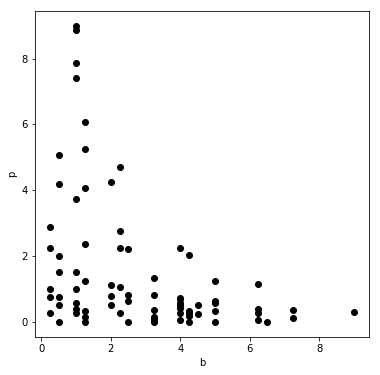
\includegraphics[width=0.3\textwidth]{pd_example}
    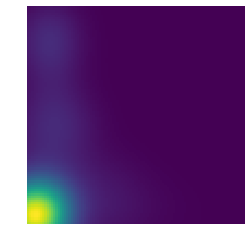
\includegraphics[width=0.3\textwidth]{rho_example}
    
\includegraphics[width=0.3\textwidth]{pi_example}
    \caption{Example PD$\rightarrow\rho\rightarrow$PI process.}
\end{figure}



\section{Spin Models}
Here we will apply the techniques of TDA to lattice spin systems. The traditional Ising model is rich in behaviour, despite being simple to describe; in two or more dimensions there is a second-order phase transition from an ordered to random state. While it is relatively easy to distinguish between these states simply by looking at the spin configurations, there exist systems in which the different states are not as readily identified. It has been demonstrated that one can use machine learning to identify phases of matter for such spin systems. We will show that this classification can also be done using persistance images built from the spin configurations, where physical characteristics of the data such as sizes of features play a central role.

As a starting point we begin with the 2d Ising model on a square lattice:
\begin{equation}
    H = -\sum_{\langle ij\rangle}s_is_j + h\sum_is_i
\end{equation}
where the sum is over all pairs of adjacent spins. Each $s_i$ takes values in $\{-1,1\}$. We will be interested in the case of no external magnetic field, $h=0$.

We take as data the physical locations of spins which all point in the same direction as the majority of spins after reaching equilibrium with a thermal bath. At very low temperatures when nearly all spins are aligned cycles are born and die very quickly, while at high temperatures features in the spins may be longer-lived.


Of interest also are spin systems in which there are topological phases, such as the $\mathbb{Z}_2$-gauged Ising model (see [\textit{Gauge fields...}, Balian et.al.]). These theories enjoy a local gauge invariance which ensures that there is spontaneous magnitization at low temperatures. Rather, in dimensions $d>2$ the phase transition is signalled by a change in the spin-spin correlation function. For $C$ a closed path in the lattice, at low temperature one finds a ``perimeter law",
\begin{equation}
    \langle\prod_C s_i\rangle \sim e^{-h(\beta)L}
\end{equation}
while at high temperatures one finds an ``area law",
\begin{equation}
    \langle\prod_C s_i\rangle \sim e^{-f(\beta)A}
\end{equation}
for $L$ the length of the path $C$ and $A$ the minimum number of plaquettes needed to span $C$. The arguments which lead to these expressions do not apply in $d=2$ (see section V.D.~of [\textit{An introduction...}, Kogut]) as the radius of convergence for the validity of the perimeter law is zero. One may also understand the special case of $d=2$ as being a consequence of the equivalence
\begin{equation}
    \Big(\text{2d }\mathbb{Z}_2\text{-gauged Ising model}\Big) = \Big( \text{1d Ising model} \Big)
\end{equation}
found by comparing the partition functions of the two models after having chosen a convenient gauge. One can, however, still hope to distinguish between high and low temperature spin configurations, as correlation lengths do change with temperature.

For $d>2$ we can hope to do more: not only identify high and low temperature configuration but also determine the critical temperature at which one shifts from a perimeter to area law. All of this occurs without the obvious spontaneous magnitization that is present in the 2d Ising model. (We will see if...) TDA techniques are powerful enough to pick up on this distinction in the topolocial ordering of the states.

\section{Models}
\subsection{Classical Ising Model}
Spins are located at the vertices of the lattice $\mathbb{Z}^d$ and the Hamiltonian is
\begin{equation}
    H = -\sum_{\langle i,j\rangle}s_is_j
\end{equation}
where $\langle i,j\rangle$ denotes all pairs of adjacent spins. The energy per spin is $-d$ at $T=0$ and 0 at $T=\infty$.
\begin{itemize}
    \item 2d: Phase transition at $T_\text{c}\approx 2.269$ from ordered to disordered. Exponential spin-spin correlation functions except for power-law at the critical point.
    \item 3d: Phase transition at $T_\text{c}\approx 4.512$ from ordered to disordered. Finite $N$: $T_\text{c}^{-1}\approx 0.2212-\frac{2.4454}{N}$ (see [0406135]). Exponential spin-spin correlation functions except for power-law at the critical point.
\end{itemize}

\begin{figure}[h]
    \centering
    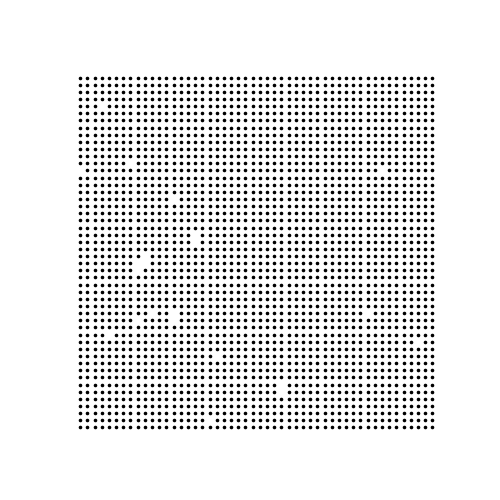
\includegraphics[width=0.3\textwidth]{ising_images/ising_T=150.png}
    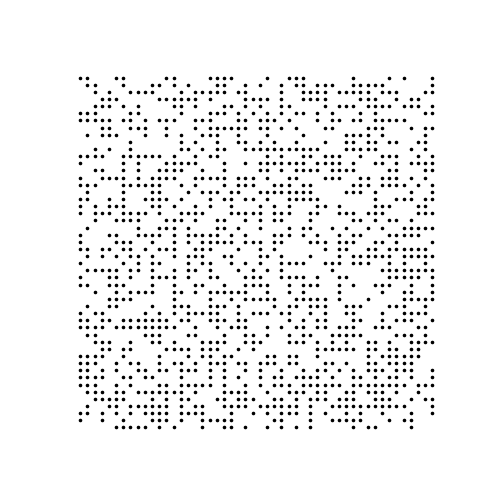
\includegraphics[width=0.3\textwidth]{ising_images/ising_T=inf.png}
    \caption{Example configurations for 2d Ising model at $T=1.5$ (left) and $T=\infty$ (right).}
\end{figure}

\subsection{Square Ice Model}
Spins are located on the edges of the cubical lattice $\mathbb{Z}^d$ and the Hamiltonian is
\begin{equation}
    H = \sum_v\Big(\sum_{i\in v}s_i\Big)^2
\end{equation}
$v\in\mathbb{Z}^d$ are the vertices and $i\in v$ is a sum over spins on edges connected to that vertex. The energy per spin is 0 at $T=0$ and 2 at $T=\infty$.
\begin{itemize}
    \item 2d \& 3d: Based on $\ev{E}$, phase transitions somewhere around $T=1\to2$. (Find in lit?)
\end{itemize}
\begin{figure}[h]
    \centering
    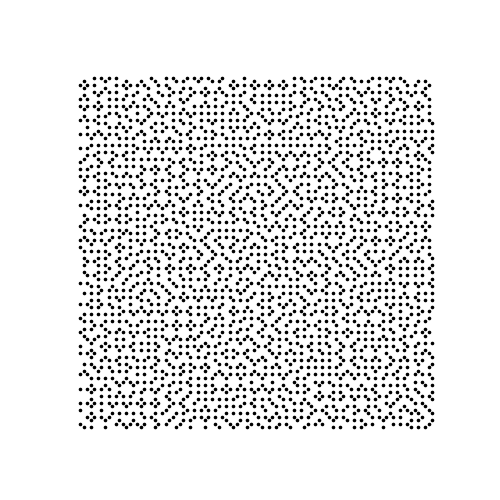
\includegraphics[width=0.3\textwidth]{squareice_images/squareice_T=0.png}
    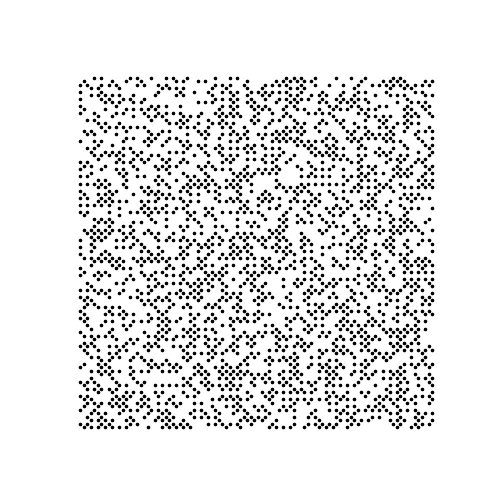
\includegraphics[width=0.3\textwidth]{squareice_images/squareice_T=inf.png}
    \caption{Example configurations for square ice model at $T=0$ (left) and $T=\infty$ (right).}
\end{figure}


\subsection{$\mathbb{Z}_2$-gauge Ising Model}
Spins are located on the edges of the cubical lattice $\mathbb{Z}^d$ and the Hamiltonian is
\begin{equation}
    H = -\sum_p\prod_{i\in p}s_i
\end{equation}
$p$ are the ``plaquettes'' and $i\in p$ is a product over the four spins around the edges of the face. The energy per spin is $\frac{1-d}{2}$ at $T=0$ ($dN^d$ spins and $\binom{d}{2}N^d$ plaquettes) and 0 at $T=\infty$.
\begin{itemize}
    \item 2d: No phase transition. Can still hope to classify $T=0$ vs $T=\infty$.
    \item 3d: No spontaneous magnetization. Phase transition at $T_\text{c}\approx??$ from perimeter- to area-law correlation functions. (Couldn't find value of $T_\text{c}$ in lit... judging from $\ev{E}$ seems to be around 1.)
\end{itemize}
\begin{figure}[h]
    \centering
    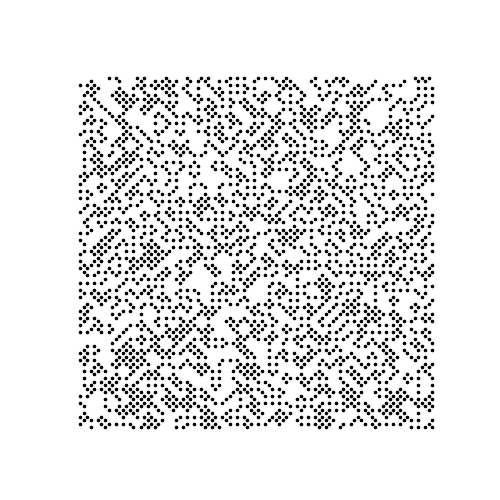
\includegraphics[width=0.3\textwidth]{gauged_images/gauged_T=0.png}
    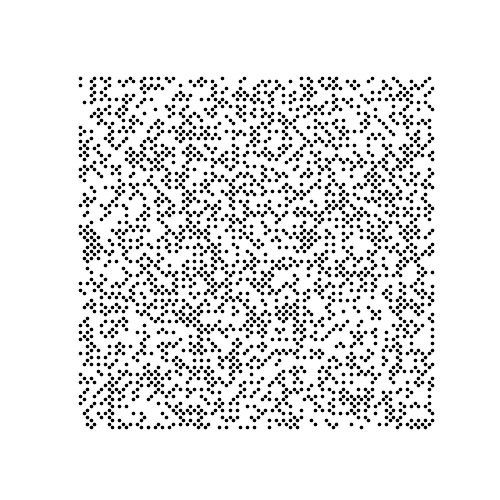
\includegraphics[width=0.3\textwidth]{gauged_images/gauged_T=inf.png}
    \caption{Example configurations for gauged Ising model at $T=0$ (left) and $T=\infty$ (right).}
\end{figure}


\section{Results}
(TO DO:) Apply logreg trained on square-lattice Ising model to triangular-lattice Ising model (critical temperature is known).

(TO DO:) For $k$-means classification, determine best value of $k$ (should be two!). Perhaps can show that for those models without a phase transition (e.g.~2d gauged Ising model) that $k=1$ is appropriate?

(TO DO:) Near $T_\text{c}$ we expect the characteristic scale-invariance of critical phenomena to be evident in the persistance diagrams/images. By considering temperatures close to $T_\text{c}$ we hope to find signatures of the diverging correlation length in the derived topological data.


\subsection{2d Classical Ising Model}
Used Wolff cluster algorithm to sample configurations weighted by Boltzmann factor. For each temperature in $\{1.00,1.05,1.10,\ldots,3.50\}$ 500 simulations were run, washing the grid until each spin is flipped an average of 20 times.

The logistic regression uses the number of short-lived cycles which are born early to classify configurations into two phases (roughly it counts the number of tiny islands of minority spins).

\begin{figure}[h]
    \centering
    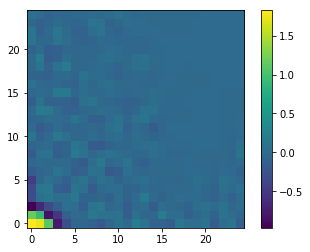
\includegraphics[width=0.32\textwidth]{ising_images/logreg_2d_ising}
    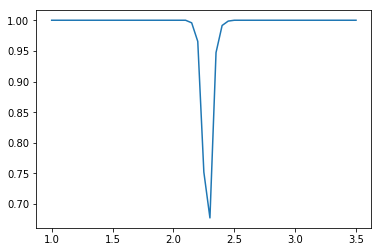
\includegraphics[width=0.32\textwidth]{ising_images/logreg_acc_2d_ising}
    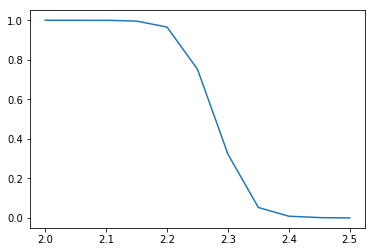
\includegraphics[width=0.32\textwidth]{ising_images/logreg_avg_2d_ising}
    \caption{Left: coefficients for logreg. Center: accuracy on testing data. Right: average classification on testing data (binned). The cross-over point gives an estimate for the critical temperature, $T_\text{c}\approx 2.2796$.}
\end{figure}

(Unsupervised!) $k$-means clustering separates $H_1$ persistence images into two clusters and gives an estimate of $T_\text{C}=2.3246$.

\begin{figure}[h]
    \centering
    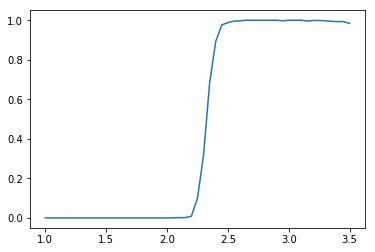
\includegraphics[width=0.32\textwidth]{ising_images/kmeans_avg_2d_ising}
    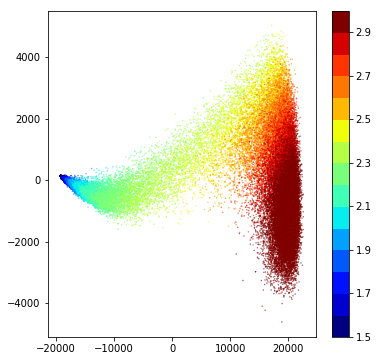
\includegraphics[width=0.32\textwidth]{ising_images/pca_2d_ising}
    \caption{Left: average cluster number on testing data (binned). The cross-over point gives an estimate for the critical temperature, $T_\text{c}\approx 2.3246$. Right: PCA on persistence images, showing clear distinction between phases.}
\end{figure}

Can repeat all of the above on $H_0$ persistence images, giving similar results.

\subsection{2d Square-ice Model}



\end{document}